%
% File acl2014.tex
%
% Contact: giovanni.colavizza@epfl.ch
%%
%% Based on the style files for ACL-2013, which were, in turn,
%% Based on the style files for ACL-2012, which were, in turn,
%% based on the style files for ACL-2011, which were, in turn, 
%% based on the style files for ACL-2010, which were, in turn, 
%% based on the style files for ACL-IJCNLP-2009, which were, in turn,
%% based on the style files for EACL-2009 and IJCNLP-2008...

%% Based on the style files for EACL 2006 by 
%%e.agirre@ehu.es or Sergi.Balari@uab.es
%% and that of ACL 08 by Joakim Nivre and Noah Smith

\documentclass[11pt]{article}
\usepackage{acl2014}
\usepackage{times}
\usepackage{url}
\usepackage{latexsym}
\usepackage{graphicx}
\usepackage{subcaption}

%\setlength\titlebox{5cm}

% You can expand the titlebox if you need extra space
% to show all the authors. Please do not make the titlebox
% smaller than 5cm (the original size); we will check this
% in the camera-ready version and ask you to change it back.


\title{Amazon cell phone evaluation platform}

\author{Marion Kramer\\
  {\tt marion.kramer@epfl.ch} \\\And
  Alexandre Rassinoux \\
  {\tt alexandre.rassinoux@epfl.ch} \\\And
Kristina Satara \\
{\tt kristina.satara@epfl.ch} \\}

\date{18.12.2017}

\begin{document}
\maketitle
\begin{abstract}
Reviews help when making decision which product to buy, as they give possible customers personal experience and more product details. Since customers usually invest some time to studying the reviews and ratings before buying specific products from Amazon, we decided to create evaluation platform which would help the users decide about purchasing the product by giving them insight into  downsides and advantages of various brands based on the reviews. The aim of this project is to analyze reviews of different brand of Amazon cell phone products and based on the reviews to decide which of the features are important for specific brands of cell phones. For this we use natural language processing techniques, such as tf-idf matrix, ...  and Latent Dirichlet Allocation.
\end{abstract}


\section{Introduction}
Sentiment analysis, also known as opinion mining or emotion AI, is important part of natural language processing. The subject of the study is the attitude or the emotion behind certain text. The purpose of sentiment analysis is to determine weather text content is neutral, positive or negative towards some topic. 

Data used for this project is collected from Amazon, during the period of few years. Most of the data is collected between 2012 and 2014, as shown in figure 2. Each of the reviews has also ratings that are used for ground truth. The ratings are based on 5-star system, where 5 is highest and 1 is lowest rating. Distribution of the ratings is J-distribution with highest number of 5-star reviews, and it is shown in figure 1. After purchasing some of the products customers are asked to give their review and rating, which are further subject to sentiment analysis in our project. 



\begin{figure}[h!]
  \centering
    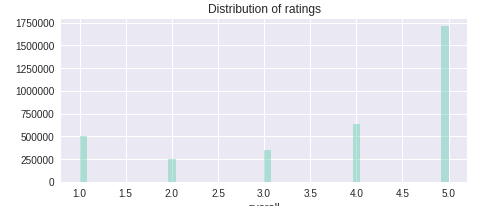
\includegraphics[width=\linewidth]{ratingDistribution.png}
  \caption{Distribution of the ratings in reviews}
  \label{fig:ratingDistribution}
\end{figure}


\begin{figure}[h!]
  \centering
    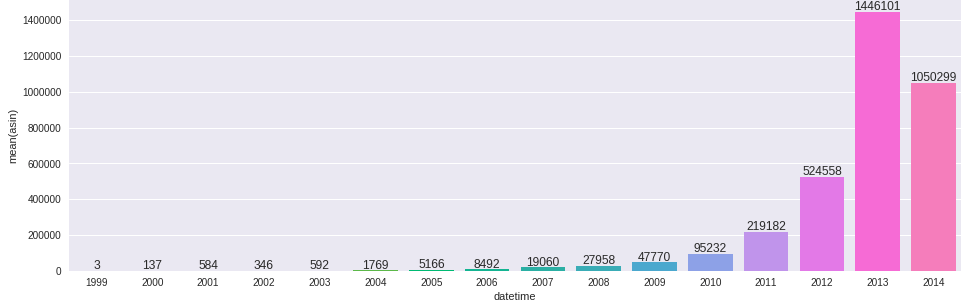
\includegraphics[width=\linewidth]{reviewsByTime.png}
  \caption{Number of reviews during time}
  \label{fig:reviewsByTime}
\end{figure}


\section{Related work}
Natural language processing is interesting and popular area of research, thus there are many papers regarding this topic. As Amazon is widely used platform, it has gained much reviews in the past few years. We focused on the cell phone reviews, and we found papers and which gave different approaches and conclusions. GIVE REFERENCES AND EXAMPLES.. In this paper they took this approach, etc etc.


\section{Data Collection}
We used dataset provided by Amazon for this project. Dataset consists of two json files - one containing the reviews, and another providing metadata about the products. Given below are the fields provided in the datasets:

\begin{itemize}
  \item Reviewer's ID
  \item ID of the product reviewed
  \item Name of the reviewer
  \item Text of the review
  \item Rating given
  \item Summary of the review
  \item Time of the review
  \item Price in euros
  \item Url of the product image
  \item Brand name
  \item Category of the product
\end{itemize}

We merged these two files for our further data analysis. Also we transformed the data in order to improve the speed of loading and processing this dataset in our python notebook. As this dataset was incomplete, we decided to enrich it with additional dataset from Kaggle platform. This is public dataset from GSMArena and it contains more than 8000 phones specifications.


\section{Dataset Description with Summary Statistics}
TODO: Explain step by step everything from the notebook. Add some more pictures. 

\begin{figure}[h!]
  \centering
    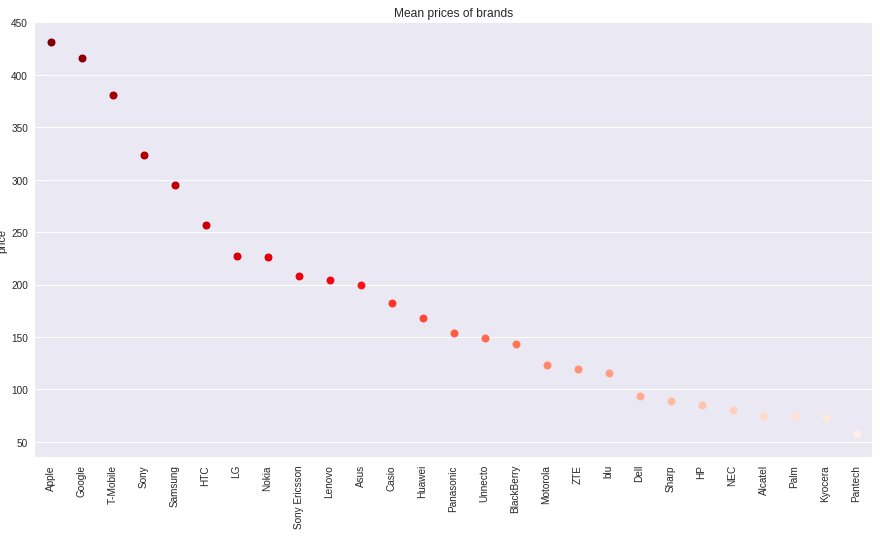
\includegraphics[width=\linewidth]{meanPrices.png}
  \caption{Mean prices per brand}
  \label{fig:meanPricePerBrand}
\end{figure}




\section{Methods}
Methods with math and description of main algorithm
Explain ft-idf, LDA, and our algorithm. 

\section{Results and Findings}
Elaborate the results about the interesting words into more details. 


\section{Conclusion}
This platform uses reviews and extracts meaningful information from it, and then evaluates certain cell phone brand based on these reviews. We use sentiment analysis to classify each of the reviews (and it's parts) as good or bad. Based on this we describe and evaluate specific brands. 


\begin{thebibliography}{}

\bibitem[\protect\citename{Aho and Ullman}1972]{Aho:72}
Alfred~V. Aho and Jeffrey~D. Ullman.
\newblock 1972.
\newblock {\em The Theory of Parsing, Translation and Compiling}, volume~1.
\newblock Prentice-{Hall}, Englewood Cliffs, NJ.

\bibitem[\protect\citename{{American Psychological Association}}1983]{APA:83}
{American Psychological Association}.
\newblock 1983.
\newblock {\em Publications Manual}.
\newblock American Psychological Association, Washington, DC.

\bibitem[\protect\citename{{Association for Computing Machinery}}1983]{ACM:83}
{Association for Computing Machinery}.
\newblock 1983.
\newblock {\em Computing Reviews}, 24(11):503--512.

\bibitem[\protect\citename{Chandra \bgroup et al.\egroup }1981]{Chandra:81}
Ashok~K. Chandra, Dexter~C. Kozen, and Larry~J. Stockmeyer.
\newblock 1981.
\newblock Alternation.
\newblock {\em Journal of the Association for Computing Machinery},
  28(1):114--133.

\bibitem[\protect\citename{Gusfield}1997]{Gusfield:97}
Dan Gusfield.
\newblock 1997.
\newblock {\em Algorithms on Strings, Trees and Sequences}.
\newblock Cambridge University Press, Cambridge, UK.

\end{thebibliography}

\end{document}
